\section{Methodology}

The Evolutionary Neuroplastic Agent (ENA) architecture pivots completely on two interconnected heuristic values: Trust and Plasticity.

\subsection{Agent Initialization}
We maintain a population of $N=20$ independent specialists. Each individual specialist governs a lightweight Multi-Layer Perceptron comprising dense layers sized $(4, 2, |\mathcal{A}|)$ equipped with orthogonal initialization and ReLU activation. At the start of an episodic run, a single ``Active Specialist" is selected from the population to act upon the environment. The selection is dictated probabilistically during training by an exploration rate $\epsilon = 0.20$, and governed entirely by maximum archived \textit{Trust} rankings during test-time meta-adaptation.

\subsection{Trust Dynamics and Plasticity Formulations}
At the termination of an episode, the agent assesses the accumulated episodic reward $R \in [0, 500]$. Operating strictly as a non-gradient update, the agent mathematically penalizes or retains the active specialist by quantifying a failure signal, defined as the Trust Decay factor $D(R) \in [0.1, 1.0]$. The active specialist's unnormalized Trust score $T$ updates autoregressively:
\begin{equation}
    T_{t+1} = (1 - D(R_t)) T_t + D(R_t) R_t
\end{equation}
Consequently, an optimal decay rate $D=0.1$ gently smooths historical rewards, whereas a catastrophic failure rate $D=1.0$ instantly plunges the specialist's Trust exactly to the penalized $R_t$, ensuring it will be instantly abandoned in the subsequent sequence.

Simultaneously, the global \textit{Plasticity} variable defines the percentage of the remaining population that will be evaluated and mutated in response to the current episode's performance. Because exploration fundamentally mirrors trust failure, the defined Plasticity search volume $\mathcal{P}(R)$ is mathematically identical to the evaluated performance drop ($\mathcal{P}(R) \equiv D(R)$), linking exploration effort continuously to survival urgency. The shared heuristic algorithms evaluated for deriving $D(R)$ and $\mathcal{P}(R)$ are compared across two configurations:

\subsubsection{Fuzzy-logic Configuration (ENA-01)}
The fuzzy variant utilizes dynamic percentiles derived from a rolling reward history $H$. Let $P_{20}$ and $P_{90}$ denote the 20th and 90th percentiles of $H$.
\begin{equation}
    D_{fuzzy}(R) =
    \begin{cases}
        0.1 & \text{if } R \ge P_{90} \\
        1.0 & \text{if } R \le P_{20} \\
        1.0 - 0.9 \left( \frac{R - P_{20}}{P_{90} - P_{20} + 10^{-8}} \right) & \text{otherwise}
    \end{cases}
\end{equation}

\begin{figure}[htbp]
\centerline{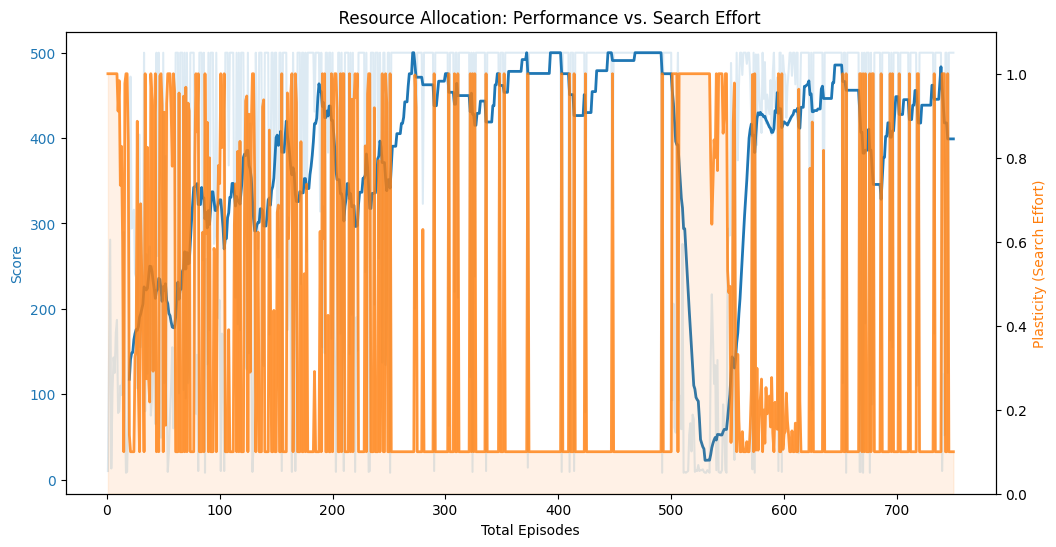
\includegraphics[width=\linewidth]{images/plasticity_ena_01.png}}
\caption{Plasticity search effort and algorithmic response mapped against the episode score average for the Fuzzy-Logic ENA-01 configuration. Spikes indicate triggered evolutionary search due to trust failure.}
\label{fig:plasticity}
\end{figure}

\subsubsection{Quadratic Ratio Configuration (ENA-02)}
The strictly mathematical variant derives loss squarely against the absolute extrema observed, clipping and penalizing failures quadratically:
\begin{equation}
    D_{quad}(R) = \min \left(1.0, \max \left(0.1, \left( \frac{R_{max} - R}{R_{max} - R_{min} + 10^{-8}} \right)^2 \right)\right)
\end{equation}

\subsection{Competitive Hall of Fame (Specialist Archive)}
To protect highly-skilled specialists, ENA regulates a structurally constrained Hall of Fame archive capped at a maximum of $K=5$ distinct specialists. This deliberate bottleneck enforces extreme genetic selectivity, ensuring only the most versatile behavioral archetypes survive long-term. An active specialist only earns induction if its performance achieves a statistically significant Z-score relative to the active population: $Z = (T_{old} - \mu_{T}) / (\sigma_{T} + 10^{-8})$. We dynamically lower induction barriers during periods of high environmental flux (high Plasticity) according to the threshold boundary: $Z_{req} = 1.5 \times (1.0 - (\text{Plasticity} \times 0.5))$.

To prevent early-discovered specialists from permanently dominating the archive, we apply an ``age-of-discovery'' memory decay mechanism. At every evolutionary check, the recorded induction Z-score of each archived specialist decays multiplicatively: $Z_{stored} \leftarrow Z_{stored} \times 0.995$. This ensures that archaic specialists gradually become vulnerable to replacement by stronger current-generation candidates, implementing an active form of bounded forgetting that prevents archive stagnation.

Once successfully evaluated for induction, a genetic similarity constraint computationally measures the flattened cosine similarity of the neural weights between the candidate and existing archive members $S_{cos\_sim} = \frac{W_a \cdot W_b}{\|W_a\|\|W_b\| + 10^{-8}}$. If two specialists are effectively identical genetically ($S_{cos\_sim} \ge 0.95$), the newer iteration battles its twin specifically based entirely on comparative Z-scores. This niche protection mechanism preserves the distinct uniqueness of isolated physics environments inside the archive without replacing structurally unique behaviors.

\subsection{Evolutionary Search Steps}
If the computed $D(R)$ rises above $0.1$, indicating the baseline trust is failing within a non-stationary physics shift, an evolutionary step is forcefully triggered. A fixed generational strategy budget governs how the next population is constructed: the top 20\% of specialists by Trust score are preserved as elites; 30\% of the new generation is produced by mutating elite parents via $\mathcal{N}(0, 0.1)$ Gaussian noise applied to a sparse 1\% of synaptic connections; a further 30\% is produced by crossover between randomly paired elites, applying a 50\% uniform random binary weight-mask per synaptic layer; and the remaining 20\% are entirely fresh randomly-initialized individuals injected to protect population-level genetic diversity. Additionally, when a catastrophic failure is detected, the Trust scores of all non-elite specialists are not reset to zero but are instead re-anchored to the dynamic historical mean $\mu_{history} = \text{mean}(H)$, preserving relative competitive rankings while preventing stale specialists from falsely dominating.
